\documentclass{beamer}
\usetheme{Warsaw}
\useinnertheme{circles}
\useoutertheme[subsection=false]{smoothbars}
\usepackage[utf8x]{inputenc}
\usepackage[czech]{babel}
\usepackage[T1]{fontenc}
\usepackage{listings}
\usepackage{tikz}
\lstset{basicstyle=\tiny\ttfamily}
\logo{
\includegraphics[height=0.5cm]{brmlab.pdf}}

\begin{document}

\AtBeginSection[]
{
  \begin{frame}
    \frametitle{Outline}
    \tableofcontents[currentsection]
  \end{frame}
}

\title{brmiversity: Umělá inteligence \\ a teoretická informatika}
\subtitle{Přednáška č. 11}
\author{Petr Baudiš $\langle${\tt pasky@ucw.cz}$\rangle$}
\institute{
	brmlab 2011\\
	\vskip 1ex
	\pgfdeclareimage[height=4ex]{ccbysa}{by-sa.pdf}
	\pgfuseimage{ccbysa}
}
\date{}
\frame{\titlepage}

\section{Neuronové sítě}

\subsection{}
\begin{frame}{Samoorganizace pomocí ANN}
\begin{itemize}
\item Umělé neurony (``výpočetní krabičky'') \\ dostávají vstupy (čísla) a na jejich \\ základě generují výstup (číslo)
\item Dnes: Chceme asociovat různé vstupy s různými neurony
\end{itemize}
\begin{tikzpicture}[remember picture,overlay]
  \node [xshift=-4.5cm,yshift=-4.5cm,above right] at (current page.north east)
    {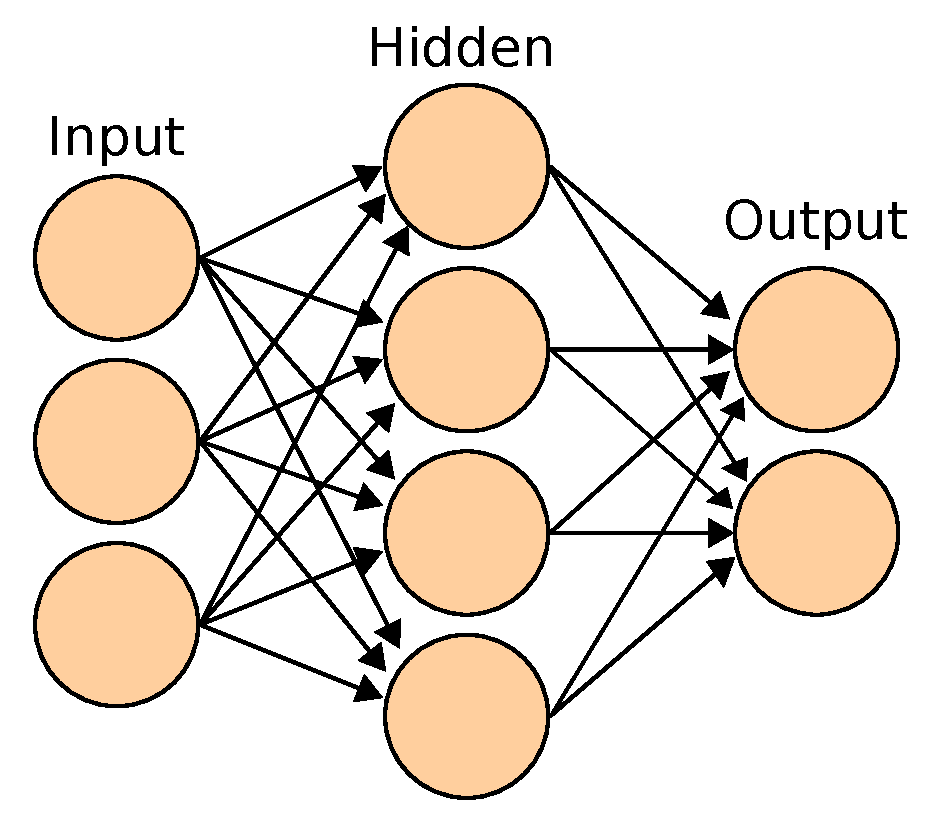
\includegraphics[width=4cm]{ANN.pdf}};
\end{tikzpicture}
\end{frame}

\subsection{}
\begin{frame}{Kohonenova mapa}
\begin{itemize}
\item Fonetický psací stroj, ekonomická data
\item Organizace, princip, učení
\end{itemize}
\end{frame}

\subsection{}
\begin{frame}{Ojův algoritmus}
\begin{itemize}
\item PCA pomocí ANN
\end{itemize}
\end{frame}

\subsection{}
\begin{frame}{Další metody samoorganizace}
\begin{itemize}
\item Laterální inhibice, ART, RBF
\end{itemize}
\end{frame}

\subsection{}
\begin{frame}{Otázky?}
\begin{center}
Příště: Modulární, hierarchické a hybridní modely.
\end{center}
\end{frame}

\section{Adaptivní agenti}

\subsection{}
\begin{frame}{Etologické modely}
\begin{itemize}
\item Jak se chovají zvířátka
\end{itemize}
\end{frame}

\subsection{}
\begin{frame}{Populační dynamika}
\begin{itemize}
\item Jak se množí a umírají
\end{itemize}
\end{frame}

\subsection{}
\begin{frame}{Otázky?}
\begin{center}
Příště: Reprezentace znalostí.
\end{center}
\end{frame}

\section{Evoluční algoritmy}

\subsection{}
\begin{frame}{Koevoluce}
\begin{itemize}
\item Paralelní vývoj problému i řešení
\item Jako paraziti --- červená královna
\end{itemize}
\end{frame}

\subsection{}
\begin{frame}{Otevřená evoluce}
\begin{itemize}
\item Strop fitness je nekonečno
\item Brmlife
\end{itemize}
\end{frame}

\subsection{}
\begin{frame}{Pravděpodobnostní model GA}
\begin{itemize}
\item Opět trocha suché teorie, jak GA funguje
\item Vzorečky
\item Jak GA funguje? Stejně nevíme!
\end{itemize}
\end{frame}

\subsection{}
\begin{frame}{Otázky?}
\begin{center}
Příště: Hrst aplikací.
\end{center}
\end{frame}

\section{Složitost}

\subsection{}
\begin{frame}{Třídy složitosti}
\begin{itemize}
\item Rekapitulace --- P, NP, PSPACE, EXPTIME
\end{itemize}
\end{frame}

\subsection{}
\begin{frame}{Míry složitosti}
\begin{itemize}
\item Polynomiální hierarchie
\end{itemize}
\end{frame}

\subsection{}
\begin{frame}{Savičova věta}
\begin{itemize}
\item TODO
\end{itemize}
\end{frame}

\subsection{}
\begin{frame}{Konstruovatelné funkce}
\begin{itemize}
\item TODO
\end{itemize}
\end{frame}

\subsection{}
\begin{frame}{Věty o zrychlení a mezerách}
\begin{itemize}
\item TODO
\end{itemize}
\end{frame}

\subsection{}
\begin{frame}{Hierarchie tříd složitosti}
\begin{itemize}
\item TODO
\end{itemize}
\end{frame}

\subsection{}
\begin{frame}{Otázky?}
\begin{center}
Příště: Pseudopolynomiální a aproximační algoritmy.
\end{center}
\end{frame}

\subsection{}
\begin{frame}{Děkuji vám}
\begin{center}
{\bf pasky@ucw.cz}

\vskip 6ex

Příště: Umělá inteligence a adaptivní agenti (reprezentace znalostí). \\
	Neuronové sítě.
	Evoluční algoritmy. \\
	Vyčíslitelnost (algoritmicky nerozhodnutelné problémy).
\end{center}
\end{frame}

\end{document}
